% beautiful title slides in Beamer
% Model 2
% latex-beamer.com

\documentclass[aspectratio=169]{beamer}

%\definecolor{fcfm-red}{rgb}{255, 24, 33}
%\definecolor{fcfm-gray}{rgb}{0.6, 0.7, 0.7}
\definecolor{fcfm-gray}{rgb}{0.44313, 0.48245, 0.49803}
\definecolor{fcfm-red}{rgb}{1, 0.0941, 0.1294}
\definecolor{fcfm-blue}{rgb}{0.1294, 0.0941, 1}

\setbeamertemplate{background}
{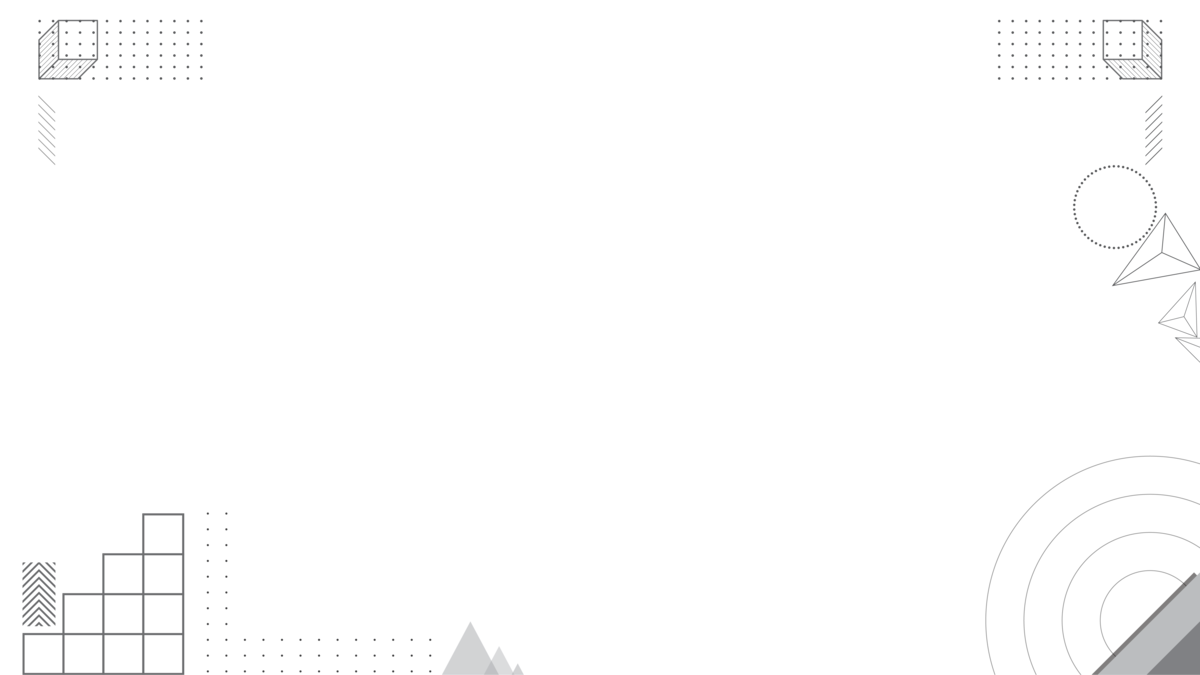
\includegraphics[width=\paperwidth,height=\paperheight,keepaspectratio]{Background 2.png}}
\usetheme{Bergen}
\usecolortheme[named=fcfm-red]{structure}
%\setbeamertemplate{footline}[text line]{%
%  \parbox{\linewidth}{\vspace*{-8pt}\hfill 
\includegraphics[width=4cm]{logos/die}}}
\setbeamertemplate{navigation symbols}{}

% Remove navigation bar
\setbeamertemplate{navigation symbols}{}

% Tikz package
\usepackage{tikz}
\usetikzlibrary{positioning}

\graphicspath{ {./img/} }

\usetheme{Bergen}

\begin{document}

%%%%%%%%%%%%%%%%%%%%%%%%%%%%%%%%%%%%%%%%%%%%%%%%%%%%%%%%%%%%%%%%%%%%%%%%%%%%%%%%%%%%%%%%
%%%%%%%%%%%%%%%%%%%%%%%%%%%%%%%%%%%%%%%%%%%%%%%%%%%%%%%%%%%%%%%%%%%%%%%%%%%%%%%%%%%%%%%%

\begin{frame}

\LARGE EL4112 Proyecto 2 \\
\large Cristóbal Allendes

\begin{tikzpicture}[overlay,remember picture]
\node[left=0.1\linewidth] at (current page.-23){
    
\includegraphics[width=4cm]{logos/die}
};
\end{tikzpicture}

\end{frame}

%%%%%%%%%%%%%%%%%%%%%%%%%%%%%%%%%%%%%%%%%%%%%%%%%%%%%%%%%%%%%%%%%%%%%%%%%%%%%%%%%%%%%%%%
%%%%%%%%%%%%%%%%%%%%%%%%%%%%%%%%%%%%%%%%%%%%%%%%%%%%%%%%%%%%%%%%%%%%%%%%%%%%%%%%%%%%%%%%

\begin{frame}

\frametitle{Características de la implementación}

\begin{itemize}
	\item Desarrollo modular $\rightarrow$ Permite añadir funcionalidades.
	\item Modulación $\rightarrow$ Se implementaron 256-FSK y 16-FSK, pero
	se usó 256-FSK.
	\item Codificación de fuente $\rightarrow$ Códigos de Huffman.
	\item No se implementó codificación de canal.
\end{itemize}

\end{frame}

%%%%%%%%%%%%%%%%%%%%%%%%%%%%%%%%%%%%%%%%%%%%%%%%%%%%%%%%%%%%%%%%%%%%%%%%%%%%%%%%%%%%%%%%
%%%%%%%%%%%%%%%%%%%%%%%%%%%%%%%%%%%%%%%%%%%%%%%%%%%%%%%%%%%%%%%%%%%%%%%%%%%%%%%%%%%%%%%%

\begin{frame}

\frametitle{Diagrama de bloques}

\begin{figure}[H]
	\centering
	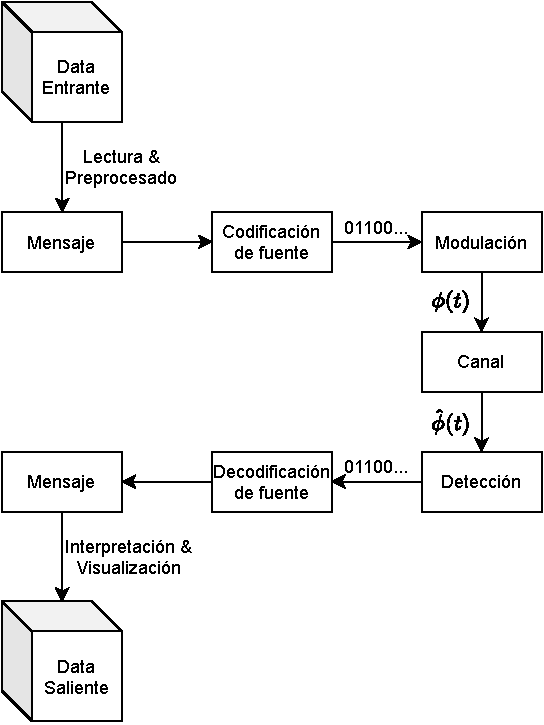
\includegraphics[width=.75\linewidth]{p2-blocks.pdf}
\end{figure}

\begin{itemize}
	\item Data $\rightarrow$ Texto o imágenes (la diferencia es el preprocesado).
	\item 
\end{itemize}

\end{frame}

%%%%%%%%%%%%%%%%%%%%%%%%%%%%%%%%%%%%%%%%%%%%%%%%%%%%%%%%%%%%%%%%%%%%%%%%%%%%%%%%%%%%%%%%
%%%%%%%%%%%%%%%%%%%%%%%%%%%%%%%%%%%%%%%%%%%%%%%%%%%%%%%%%%%%%%%%%%%%%%%%%%%%%%%%%%%%%%%%

\end{document}
